
\ifx\isEmbedded\undefined

\documentclass[12pt,a4paper]{report}
\usepackage[bottom=2.5cm,left=2.0in,right=2.5cm]{geometry}

% FONT RELATED
\usepackage{times} %Move to times font
\usepackage[labelfont=bf,textfont=it]{caption}

% LINKS, PAGE OF CONTENT, REF AND CROSS-REF, HEADERS/FOOTERS
\usepackage{footmisc}
\usepackage{hyperref}
\usepackage{bookmark}
\usepackage{fancyhdr}
%\usepackage{nameref}

% FIGURES, GRAPHICS, TABLES
\usepackage{graphicx}
\usepackage{parskip}
\usepackage{tocloft}
\usepackage{array}
\renewcommand{\cftfigfont}{Figure }
\renewcommand{\cfttabfont}{Table }
\usepackage{longtable}

%\newlength{\mylen}
%\renewcommand{\cftfigpresnum}{\figurename\enspace}
%\renewcommand{\cftfigaftersnum}{:}
%\settowidth{\mylen}{\cftfigpresnum\cftfigaftersnum}
%\addtolength{\cftfignumwidth}{\mylen}






%\usepackage{subfigure}
\usepackage{wrapfig}
\usepackage{caption}
\usepackage{subcaption}


% COLOURS, TEXT AND FORMATTING
%\usepackage[left=2.0in,right=0.5in]{geometry}

\usepackage{array}
\usepackage{color}
\usepackage{setspace}
\usepackage{longtable}
\usepackage{multirow}


% ADVANCED MATHS, PSEUDO-CODE
\usepackage{amsmath}
\usepackage{amsfonts}
\usepackage{alltt}
%\usepackage{algorithm2e}
\usepackage{algorithmicx}
\usepackage{algorithm}
\usepackage{algpascal}
\usepackage{algc}
\usepackage{algcompatible}
\usepackage{algpseudocode}
\usepackage{linegoal}

% BIBLIOGRAPHY
\usepackage{natbib}
%\usepackage[authoryear]{natbib}
%\usepackage{harvardnat}
\bibpunct{(}{)}{;}{a}{}{,}
%\usepackage{bibentry}
%\nobibliography*



% LINE NUMBERS
%\usepackage{lineno}
%\linenumbers

% USE IN DISSERTATION:

% MARGINS
%\setlength{\oddsidemargin}{2.0in}
%\setlength{\evensidemargin}{0.5in}
%\setlength\headsep{2.5in}

% TEXT
\setlength\textheight{9.5in}
\setlength\textwidth{5.1in}

% indent at each new paragraph
\setlength\parindent{1.0cm}
%\setlength\parindent{0.5cm}

%\setlength{\parskip}{10.5ex}

\setlength\topmargin{-0.2in}

% 1.5 spacing:
\renewcommand{\baselinestretch}{1.5}
%\renewcommand{\baselinestretch}{1.3}
%\fontsize{15}{15}\selectfont

% USE IN REPORT:

%\setlength\oddsidemargin{1cm}
%\setlength\evensidemargin{0.3in}
%%\setlength\headsep{2.5in}
%
\setlength\textheight{9.0in}
%\setlength\textwidth{5.5in}
%
%% indent at each new paragrapg
%\setlength\parindent{0.5cm}
%
%%\setlength{\parskip}{10.5ex}
%
%\setlength\topmargin{-0.2in}

%\newcommand{\HRule}{\rule{\linewidth}{0.5mm}}
\newcommand{\HRule}{\rule{\linewidth}{0.0mm}}

% Color definitions (RGB model)
\definecolor{color-comment}{rgb}{0.1, 0.4, 0.1}
\definecolor{color-variable}{rgb}{0.000,0.000,0.616}
\definecolor{color-question}{rgb}{0.4, 0.0, 0.0}
\definecolor{color-new}{rgb}{0.2, 0.4, 0.8}

\newcommand*{\Let}[2]{\State #1 $\gets$
\parbox[t]{\linegoal}{#2\strut}}

\newcommand*{\LongState}[1]{\State
\parbox[t]{\linegoal}{#1\strut}}

\graphicspath{{../images/}}
\begin{document}
%\maketitle
\fi

%**************************************************************************
%**************************************************************************
\chapter{Introduction}
\label{cha:introduction}
Cloths not only reflect a persons social status but also act as a medium of communication in peoples daily life\Citep{barnard2002fashion}. In general, modern cloth making process involves five steps\Citep{margolis1964complete}, choose a style, measure the body of a customer, adjust cloth patterns, assemble patterns and final try-on. For bespoke clothing, each pattern is cut slightly larger than desired size, before final assembling, patterns will be loosely stitched together and put onto the customer to further trim off the excess to achieve better fit. 

In fashion industry, cloth patterns are the feasible solution of a fashion design concept. It is constituted by a set of 2D outlines which are the breakdowns of a complete cloth design\Citep{rosen2004patternmaking}. Cloth design process are usually carried out on an ideal figure which is called standard body template. In order to produce textile pieces that can be assembled to form a cloth for a costumer, cloth patterns need to be adjusted to a particular size for the customer by an experienced tailor. Nowadays, cloth pattern is the most important medium in fashion industry. Almost all the cloth designs are preserved or distributed in the form of cloth patterns. Cloth pattern also provides an intuitive instruction for users to implement a cloth. Moreover, by altering certain parts of a cloth pattern, the cloth can be adjusted into any desired size for any wearer. 


\section{Cloth Making and Fashion Design}
``Fashion design is the art of the application of design and aesthetics or natural beauty to clothing and accessories. Typically, fashion refers to the phenomenon of a regular pattern of change in the prevailing mode of dress.''\Citep{steele2005encyclopedia}. In this thesis, the term ``Fashion Design'' only refers to cloth design. Cloth making is the process that transfers design concept into wearable objects. The history of cloth making follows tightly with the evolution of human. It is not known when human started to wear cloth, but the evidence shows that man start wearing cloth from 170,000 years ago\Citep{Dunn201236}. In Ancient times, clothes are usually made of natural elements such as animal skins or furs, plant leaves, bones and shells that was draped or tied onto body. The appearance of textile during the late stone age in Middle East\Citep{LYNCH30081985} not only improved both comfort and functionality of cloth at that time but also enabled human to produce wearable materials by themselves. The discovery of bone needles which can be dated to 61,000 BP\Citep{Backwell20081566} reveals the evidence of sewn textiles or leathers used to make cloth at that age. 

During Middle Ages, cloth has already become a symbol of wealth and social status. Fashion was the privilege of upper class only, who can afford to hire private dressmaker to make cloth for them\Citep{crane2012fashion}. 

Modern fashion that every one could enjoy was brought to general public by Rose Bertin, who was the dressmaker to Marie Antoinette(2 November 1755 – 16 October 1793), Queen of France. It is said that she was the first one who starts the transition from low public profile private dressmakers to a well-know fashion designers.  The cloth shop she opened in Paris had a considerable influence on Parisian style\Citep{steele1998paris}. In 1863, Ebenezer Butterick invented the first graded sewing pattern for cloth making \Citep{Millard:1919, O'Loughlin:1899}. Soon after his invention, cloth pattern became massively popular, as they made modern fashions much more easier to be accessed by the rapidly expanding lower middle class. This innovation provides a standard for fashion designs to be preserved and spread with much lower cost, moreover, it allows a design to be adapted to different human figures with ease. 

%The process of fashion design starts from an inspiration of designer. A rough and abstract sketch is created to express the concept of the design. When the design concept is confirmed by designer, more details are added to the concept to create a preview of the cloth. After that, designer selects textile materials that suits the appearance and function of the design. 

The term ``Fashion Design'' is usually refers to the process of constructing the cloth design concept and producing the samples on the standard body template. Figure\ref{figure:SBT} demonstrates a standard body template which is the ideal human body that has ideal body proportion. 

 \begin{figure}[H]
    \centering
	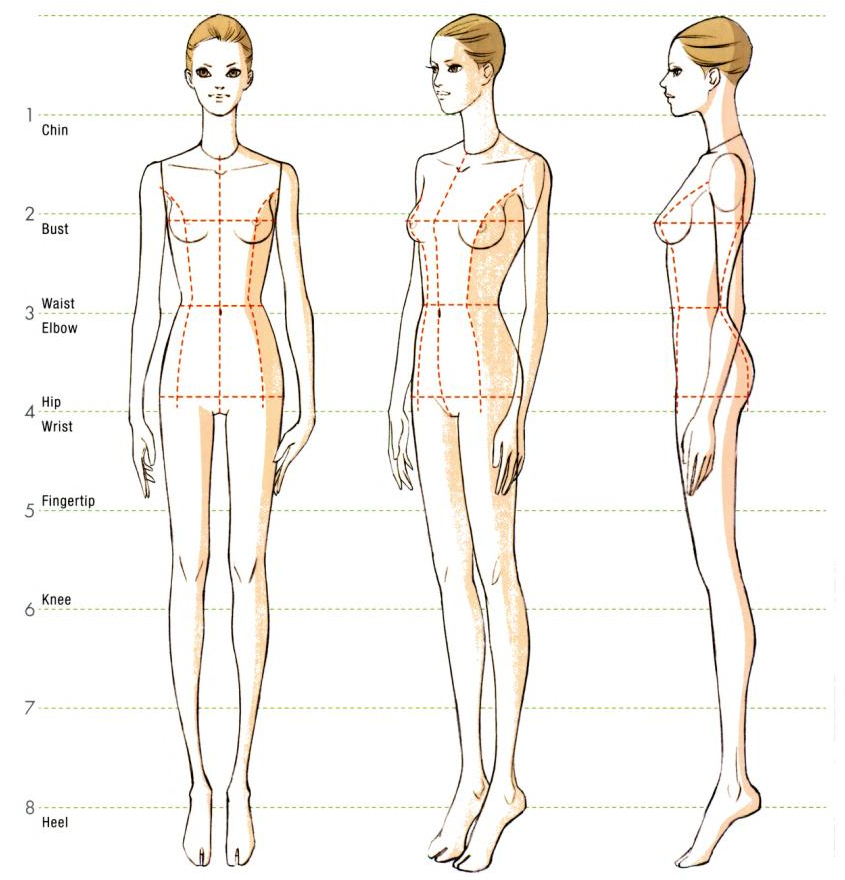
\includegraphics[width=0.9\columnwidth]{../images/cloth_design/standard_body_template}\\[1cm]
    \caption{Standard Body Template in fashion design\Citep{rosen2004patternmaking}}
    \label{figure:SBT}
\end{figure} 

 Modern fashion design process involves a five steps process to transfer a design idea into a wearable sample cloth \Citep{stecker1996fashion} :
\begin{description}
  \item[Design Inspiration and Sketches] \hfill \\
  Fashion designers constantly searching for the new idea to create new style. They record their inspiration of the new style by using rough and abstract sketches. Simple drawing allows more room for modifying and expressing their thoughts.

  \item[Fabric Selection] \hfill \\
  There are many types of textile materials with different method of interlacing and interloping fabric materials that provide different physical proprieties. Different types of textile materials also affect the appearance of cloth differently. Based on the type of cloth, designers select suitable textile materials for the design. 
  
   \item[Final Sketches] \hfill \\
  By using standard body template, colours and details such as pockets, seam lines and other accessories are added onto the sketch. The final sketch is a detailed preview of the design worn by a model. 
  
    \item[Patternmaking] \hfill \\
  Before patterns can be produced, fabrics are positioned or pinned on a dress form to reveal the structure of a garment design, this process is called ``Draping''\Citep{stecker1996fashion}, it allows designer to visually exam the design on a human body. After the design has been draped, patternmaker decomposite draped cloth design and transfer it onto paper. Both cloth details such as seams, darts, cuttings and sewing instruction are indicated on the paper pattern.
  
    \item[Samples and Flat Drawings] \hfill \\
	After paper patterns are produced, they first pinned on top of the fabric for cutting and then removed allowing fabric pieces to be sewn together. For design storage and distribution, both patterns and flat drawing are required. Flat drawing acts as a blueprint of a design which contains all the details for constructing clothes. 

\end{description}

The aforementioned fashion design process involves many iterations of transferring design concept from 2D sketches to 3D draping, then back to 2D patterns. In other words, designers expresses their idea by 2D sketch, patternmaker reconstructs the 3D cloth structure in real world and decomposites the structure back to a set of 2D patterns. Finally, 3D sample cloth is produced based on 2D patterns. Often the resulting sample cloth reveals desired modification in the 3D form of the design that, in turn, the revisions of the 2D patterns also need to be carried out. Finally the new sample is created for further inspection. This iteration continues till the final sample is signed off by designer.

After cloth design process is completed, next step is to produce cloth for customers, and ``Cloth Making'' refers to the process of producing clothes based on cloth patterns. This process is aiming for producing clothes with certain sizes for actual customers and it is constituted by four steps: 

\begin{description}
\item[Measuring] \hfill \\
Different individual has different body shapes and proportions. In order to fit a cloth to a customer, body measurements need to be extracted. This step acquires measurements of the body parts that are associated with the cloth. Tape ruler is the most common tool for performing measuring on a customer. 
\item[Pattern Grading] \hfill \\
Because cloth patterns and flat-drawing are developed on the standard body template, the size of each patterns need to be altered in order to fit a customer. Based on the measurements of customer, corresponding parts of patterns are adjusted to meet measurements. 
\item[sewing] \hfill \\
After patterns are adjusted to desired size, fabric pieces are cut out slightly large than required size. Then patterns are stitched loosely to form the initial cloth. 
\item[Try-on] \hfill \\
At this step, cloth is fitted to customer to further adjust the stitch and trim off the excess in order to achieve best fit. Finally, all the patterns are sewn together to form the final garment.
\end{description}

For the massively produced cloth, in order to make clothes that can be wore by general public, cloth patterns are scaled to several predefined sizes based on a size chart. Size chart contains body size data from a particular ethnic or group of people who shares the similar body proportion. The size chart various among different countries or areas, i.e. US Size Chart \Citep{USsizeChart2010}, UK Size Chart \Citep{UKsizeChart2005}, Euro Size Chart \Citep{ashdown2007sizing}. Table\ref{Table:Size_Chart} illustrates converting rule between different size chart and major measurements used to define cloth size in a size chart.

 \begin{figure}[H]
    \centering
	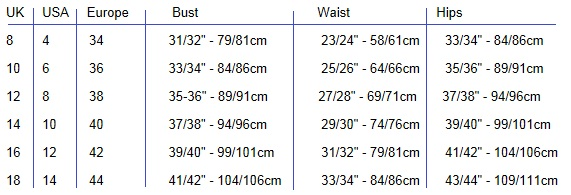
\includegraphics[width=1\columnwidth]{../images/cloth_design/size_chart}\\[1cm]
    \caption{UK, US, Euro Size Chart convert table}
    \label{Table:Size_Chart}
\end{figure} 

%Modern cloth design process requires a five steps process\Citep{stecker1996fashion} to transfer a design idea into a wearable cloth:
%
%\begin{description}
%  \item[Design Inspiration and Sketches] \hfill \\
%  Fashion designers constantly searching for the new idea to create new style. They record their inspiration of the new style by using rough and abstract sketches. Simple drawing allows more room for modifying and expressing their thoughts.
% \begin{figure}[H]
%    \centering
%	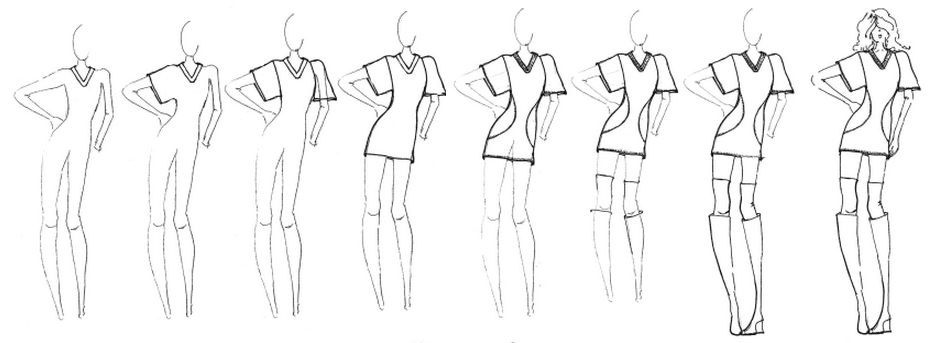
\includegraphics[width=1\columnwidth]{../images/cloth_design/design_sketch}\\[1cm]
%    \caption{Cloth concept designs\Citep{hopkins2009basics}}
%    \label{figure:weil}
%\end{figure} 
%  
%  \item[Fabric Selection] \hfill \\
%  There are many types of textile materials with different method of interlacing and interloping fabric materials that provide different physical proprieties. Different types of textile materials also affect the appearance of the cloth differently. Based on the type of the cloth, designers select suitable textile materials for the design. 
%  
%  \item[Fabric Construction] \hfill \\
%  The third etc 
%   \item[Final Sketches] \hfill \\
%  The third etc 
%    \item[Draping, Fitting and Patterns] \hfill \\
%  The third etc 
%    \item[Samples and Flat Drawings] \hfill \\
%  The third etc 
%\end{description}
%



%Clothing technique is essential to people's daily life. It has been developed for more than hundreds years. In order to produce a cloth, normally there are five steps involved in this process\Citep{margolis1964complete}, choose the style, measure the body of the customer, adjust the cloth patterns, assemble patterns, and final try-on. For bespoke clothing, before final assembling, patterns will be loosely stitched together and put onto the customer to further trim off the excess to achieve better fit. In 1863, Ebenezer Butterick invented the first graded sewing pattern for cloth making \Citep{Millard:1919, O'Loughlin:1899}. Soon after his invention, cloth pattern became massively popular, as they made modern fashions much more easier to be accessed by the rapidly expanding lower middle class. This innovation also provides a standard for fashion designs to be preserved and spread with much lower cost, moreover, a design can be adapted to different human figures with ease.

%Cloth patterns consist of a set of textile pieces which are the breakdowns of a complete garment\Citep{rosen2004patternmaking}. It is the most important medium in today's fashion industry. Almost all the cloth designs are preserved or distributed in the form of cloth patterns. Cloth pattern also provides an intuitive instruction for users to recreate a cloth to its design. Moreover, by altering certain parts of a cloth pattern, the cloth can be adjusted into any desired size for any wearer. 

%Followed with the fast development of computer hardware and computer graphic techniques, simulating clothes and clothing in virtual environment has become a hot research topic for decades. By constructing a cloth object in virtual environment, virtual clothing techniques can reproduce both visual effects and physical behaviours of textile objects. Virtual clothing is the generic term of this process\Citep{volino2000virtual}. 
%


%Virtual clothing is a research topic in the field of computer graphics for a very long time. It is the generic terms of simulating clothes and clothing in computer simulated virtual environment. It reproduces both visual features and physical behaviours of textile objects in computer simulated virtual reality \Citep{volino2000virtual}.

%In general, there are two areas utilise the virtual clothing techniques, today's fashion industry and film or game industry. 

%In the fashion industry, cloth pattern is an important medium for the storage and distribution of a cloth design. Producing, editing and visualising the cloth design pattern efficiently is crucial to the cost of the cloth production. Pattern based virtual clothing technique is able to provide an efficient tool for the cloth designer to pre-visualise and edit the cloth pattern before its production, therefore, it is widely used in the process of cloth designing.  
%
%In today's film and game industry, virtual character is an important element of the virtual environment. The costume of the virtual character plays an very important role to the expressiveness of the character. Because the design of the character and its outfit varies largely among the artists, the intuitiveness and ease-of-use of the cloth modelling tool is important to the animation artist. Geometric modelling method creates and edits the basic element of the geometrical representation of the cloth. Therefore, its simplicity and intuitiveness makes it the most popular method for cloth modelling. Operating directly on the basic geometrical element provides great controllability to the animation artists.



%In general, there are two types of methods for modelling cloth for virtual character, geometrical cloth modelling method and pattern based cloth modelling method. The geometrical modelling method creates and edits the basic geometrical element of the geometrical representation of the cloth. The simplicity of the geometrical cloth modelling method makes it the most popular method for modelling cloth for character in film, TV and gaming industry. Operating directly on the basic geometrical element provides great controllability to the animation artists.

%Pattern based cloth modelling method uses cloth patterns from fashion designers and assemble patterns together to form a complete cloth. Because pattern based cloth modelling method are more close to the real cloth making process, it requires textile engineering knowledge, tailoring expertise. It is mostly used in fashion industry as an design tool for previewing the cloth before production.

%
%
%Virtual clothing methods are capable of producing realistic cloth model. Past research on virtual clothing methods were mainly focus on modelling cloth for a single character. The current pattern based cloth modelling methods have failed to find meaningful use within animation or gaming industry because they are notoriously difficult to create and reuse especially with multiple different characters. 
%
%
%
%
%
%The construction of the computer simulated virtual environment has been studied intensively throughout the history of computer science. Now a days, interactive virtual world has become a powerful tool in many research fields. Equally important as human-being to the real world, virtual human is a fundamental component to the virtual environment. 
%
%
%Today, with the high speed development of computer hardware, realistic virtual character has been wildly used not only in research, but also in commercial production such as film, TV, and games as well as fashion industry. For the applications of the virtual character, the clothing of the virtual character is a crucial factor that directly affects their fidelity. On the other hand, in the fashion industry, virtual clothing has brought a big leap into the designing and manufacturing process. With the help of virtual clothing techniques, this traditional labour-intensive industry has been transferred into a highly automated modern industry. 
%
%Virtual clothing consists with two major tasks, cloth modelling and cloth simulation, as the area of application differs, the focus point of virtual clothing varies. For computer aided cloth design in fashion industry and automated cloth pattern cutting in garment manufacturing, the accuracy of cloth modelling and cloth simulation are crucial. However, in computer animation and gaming applications, achieving high visual fidelity is the main objective.  
%
%This thesis presents a research that focuses at modelling cloth for characters with different body proportion with high efficiency. Because the computational ability of the computer hardware has been improved significantly during the past decade, more and more characters are able to be handled in the virtual environment. Therefore, clothed virtual character in varied body shapes are necessary for the virtual environment. However, virtual clothing is such a task that involves both textile engineering knowledges, artistic expertise as well as computer graphic techniques. It has always been considered as a challenging and time-consuming task. Moreover, current virtual clothing researches mainly focus at cloth modelling or simulation for single character, the problem of fitting clothes to character with different body shapes is rarely addressed. Therefore, in order to dress multiple characters with different body proportions, the current virtual clothing method need to be performed repetitively. 
%
%However, in real world, thanks for the tailoring techniques that has been developed for centuries, an experienced tailor is able to fit a cloth design to any customer with vastly different body proportions. Moreover, in the fashion industry, one cloth design can be purchased with different sizes in order to fit different customers. Inspired by the techniques in the garment manufacturing, the virtual clothing method presented in this thesis measures the character and automatically adjusts the size of the cloth based on the measurements so that the cloth that modelled fits the character. By automated the cloth fitting process, a cloth design can be fit to a character easily. Furthermore, for the problem of dressing characters with different body proportion, only the measuring process need to performed for each character and the cloth that fits to the characters can be generated respectively. This method significantly reduced the duplication of effort when dressing characters that have different body proportion by using current virtual clothing method.

%--------------------------------------------------------------------------
\section{Virtual Clothing in Fashion Industry}
Traditional fashion design and cloth making procedure are considered as highly skilled, labour intensive process that require many iterations to complete. Followed with the advancement of computer hardware and computer graphic techniques, constructing and evaluating cloth design in virtual environment instead of actually performing the cloth making process repetitively dramatically cuts down labour and time consummation required in traditional cloth design and cloth making process. 

Virtual Clothing is the generic term of the process which constructs both visual effects and physical behaviours of textile objects\Citep{volino2000virtual}. It is the foundation of cloth CAD/CAM technologies which are widely used in fashion industry to assist the design of garment product. In terms of composition, cloth is constituted by a set of shape predetermined textile pieces which are assembled following a predefined order to cover a specific body area. The aim of virtual clothing techniques in fashion industry is to produce cloth patterns and evaluate cloth design effectively and efficiently. 

%Due to the special property of clothes and textiles, there are several issues need to be addressed during the development of virtual clothing techniques for fashion design. Firstly, textiles are soft material with low bending stiffness and high stretch and compress stiffness. Secondly, cloth patterns are assembled together following specific tailoring rule and techniques. The pattern assembling techniques also have a heavy impact to both appearance and functionality of clothes. Thirdly, although clothes are constructed from 2D cloth patterns, the quality of fit and comfort is evaluated on 3D human model.  

In order to construct cloth in a virtual environment, two fundamental requirements need to be fulfilled, 2D cloth patterns from fashion designers and 3D virtual mannequins that are used for cloth assembling and 3D evaluation. In general, four steps are involved in the process of constructing virtual cloth, 2D cloth pattern generation, assembling 2D patterns to 3D cloth, 3D cloth simulation, comfort evaluation. The process of constructing virtual cloth generally follows the procedure of the making real cloth, however, because cloth patterns are created, edited, graded and pre-visualised in virtual environment, implementing cloth design into a real cloth for evaluation can be avoided, therefore, improve the efficiency and reduce the cost of fashion design. 

There are various applications targeting to each stages of cloth design to improve the productivity of designers. 

\begin{description}
  \item[2D Pattern Editing] \hfill \\
 Computer aided cloth pattern design system such as Kaledo\Citep{Kaledo} and Cameo\Citep{WidGingerSoftware} have been widely used in various fashion brands across the world. Traditionally, cloth patterns are usually made of paper boards cut out by patternmakers. In order to make cloth for different customers with different body shapes and proportions, the standard cloth patterns need to be adjusted into different sizes by experienced tailors based on the measurements of customer. With the help of cloth pattern CAD/CAM system, creating, editing and grading cloth patterns can be performed in virtual environment. Especially in large-scale cloth production, cloth pattern CAD/CAM methods not only save the materials but also provides an intuitive and convenience approach for cloth pattern manipulation. 
     

  \item[Cloth 3D visualization] \hfill \\
  Cloth 3D visualization techniques generate 3D cloth object in virtual environment either based on 2D cloth patterns\Citep{Fontana2005609,MD,PDS} or designer's sketches\Citep{Emmanuel2007}. Traditionally, visualizing 2D cloth patterns requires the most iterations and labours in traditional fashion design process. Any changes on 3D form need to be amended on 2D patterns, and a new sample cloth needs to be produced in order to visualize the amendments. These iterations between 2D and 2D perspective consume materials and time. 3D visualization techniques eliminate these costs by creating and assembling cloth patterns in virtual environment. Cloth pattern can be edited and visualized without need of actually producing cloth from textile pieces, which saves both time, materials and labours. 
  
   \item[Virtual Try-on] \hfill \\
   Virtual try on techniques enables designers to fit cloth onto avatars with different body shapes and proportions to review the appearance, fit and degree of comfort of clothes. It also allows customers to visually try clothes without walking into local shops. Different from aforementioned virtual clothing applications which focus at cloth design on the standard body template, this type of techniques usually involves body measurements acquisition from real customers, 3D body reconstruction, cloth modelling and cloth simulation. It provides the most intuitive visual experiences of a cloth design. Moreover, thanks to the advancement of 3D scanning techniques, the body shape and its measurements can be acquired automatically from customers. Combining with the 2D pattern editing techniques, fashion designers are able to produce custom made cloth with much higher efficiency and lower costs. 

  
    \item[Textile Engineering] \hfill \\
    Textile is a type of complex structure materials which is made of fabric threads that are inter laced or looped together. Cloth simulation utilises physical models to describe mechanical and structural properties of textiles and provides an effective tool for textile engineers to create, simulate and analyse the dynamic properties of textiles constructed with various weaving techniques and materials.
    
\end{description}

%In modern fashion industry, textiles are often used within composite materials in order to achieve outstanding mechanical and structural properties or form complex shapes. 
%
%The textile modeling requirements for industrial applications are quite different from the requirements for entertainment and apparel design applications. 
%In the composites domain, cloth is 
%not allowed to freely drape over another object. it is forced into a specific predetermined shape. Composite material designers need to know if a cloth can be 
%deformed into the desired shape and, if so, what outline 
%is required to cover a specific area. Additionally, they 
%need a detailed structural analysis of the material’s 
%strength. 
%
%
%Computer-aided manufacturing places additional 
%demands on textile and apparel modeling. Industry 
%wants to automate the manufacture of clothing and 
%other textile-based products, which is extremely labor- 
%intensive. Integration of robotics into the manufacturing 
%process is expected to save significant time and money. 
%While robot manipulation of rigid objects, such as auto 
%parts, has been thoroughly studied and is well under- 
%stood, the automated manipulation of a highly flexible 
%and complex material such as cloth still presents great 
%challenges to the robotics community. Controlling a 
%robot to properly handle and place a limp object is a dif- 
%ficult problem that requires extensive study. Modeling a 
%cloth’s dynamic properties and predicting its motion in 
%reaction to applied forces are critical to solving the gen- 
%eral control problem. 
%
%Garment CAD technology is the use of computer technology to
%assist the design of garment product. Compared to other
%mechanical product, garment CAD has to address some special
%issues. Firstly, it models soft material with low bending stiffness
%rather than rigid solid objects. Secondly, garment components
%such as collar and sleeve, are assembled together following specific
%pattern-making rules which are totally different from the
%conventional assembly methods. Thirdly, while the garment is
%constructed from 2D patterns, the quality of fit is evaluated on 3D
%human models. Based on these observations, garment CAD is a
%unique research area that has attracted considerable attentions.



\section{Virtual Clothing in Computer Animation}

Differ from virtual clothing techniques in fashion industry, virtual clothing techniques in computer animation mainly aim at producing realistic appearance of 3D cloth objects. In animation, apart from the character's body and facial expression, costumes also play a very important role in acting. It is the symbol of social statue and personality of characters. 

 \begin{figure}[H]
    \centering
	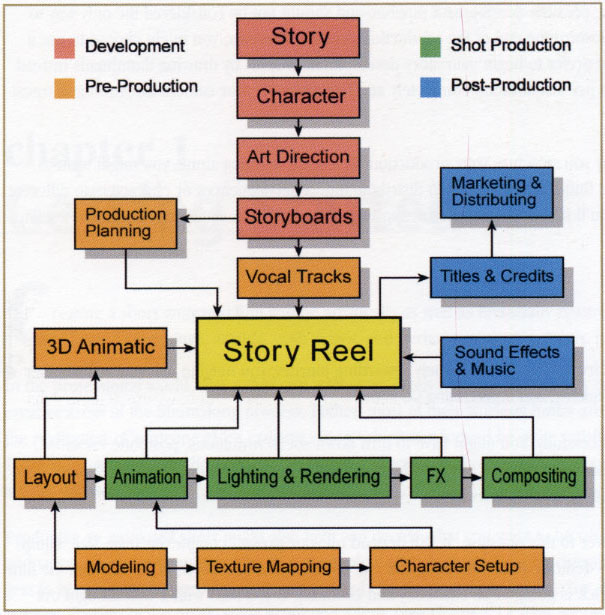
\includegraphics[width=0.9\columnwidth]{../images/animation_pipeline}\\[1cm]
    \caption{Animation production pipeline\Citep{PipelineOnline}}
    \label{Figure:pipeline}
\end{figure} 

Figure \ref{Figure:pipeline} demonstrates the production pipeline of animation film. The process of creating outfits starts from character( Character Design ) phase which is at very early stage of the development process. Outfits are designed together with characters. In the modelling stage, clothes are modelled after the completion of character modelling. At this point, animators utilise various modelling method to build 3D cloth. During character setup, deformers are assigned to character model to drive its movement. Depends on the requirement of the film, some clothes are driven by skeleton system. For realistic clothes, they are simulated by cloth simulation module. Therefore, based on the animation production pipeline, virtual clothing in computer animation is constituted by two parts, cloth modelling and cloth simulation

\subsection{Cloth Modelling}

Cloth modelling is the process of constructing geometrical shape of cloth in a virtual environment. Due to the vast variety of the character designs, the intuitiveness and controllability of cloth modelling method are crucial to animation artists. In computer animation, beside the pattern based cloth modelling method which is widely used in fashion industry, the most popular modelling method for cloth is general-purpose geometric modelling method due to its intuitiveness and ease of use. By using this method, cloth can be modelled same way as other objects are modelled such as character, building and  vehicles. Without the need of tailoring knowledge, this type of method operates directly on the basic element of the geometrical representation of clothes, therefore, it gives the user maximum controllability throughout the modelling process and the appearance of 3D cloth can be viewed throughout the entire modelling process. However, the quality of cloth model depends on the artistic scenes of its modeller. Different modeller may produce different cloth from same cloth design. Moreover, because cloth is a soft object that follows the profile of character body, it cannot be dressed onto another character which has different body shapes and proportions without major modifications. In order to modify a cloth for a different character, heavy workload is required to perform such a process.  

On the contrary, pattern based cloth modelling method operates on cloth patterns. Cloth patterns define the appearance of cloth, thus the consistency of the style of a cloth modelled different animators can be maintained. However, to form a 3D cloth from 2D cloth patterns requires expertises in tailoring and few animation artists possess such a skill. Moreover, in order to evaluate a cloth, the pattern assembling process need to be completed to form the 3D cloth and any modification that are required need to be executed on 2D cloth patterns which makes editing a cloth notoriously tedious due to the repetition of modelling process for modifying cloth patterns.   

\subsection{Cloth Simulation}

Cloth simulation is the process of reproducing dynamic behaviours of cloth objects in a virtual environment. Based on methods used for driving deformation of a cloth, in general, there are two types of cloth simulation methods used in the computer animation. 

Physical cloth simulation utilises a physical model such as mass-spring model or energy model to describe mechanical properties of a piece of cloth. By using the mechanical model developed from the real world, this method is able to reproduce realistic dynamic behaviours of clothing. However, because the detail of cloth deformation is determined by the number of the basic elements of the geometrical representation of cloth, this process requires large amount of computational power and time to generate fine detailed cloth deformation. 

Hybrid cloth simulation methods utilise other types of deformation models such as data-driven method or geometrical modelling method to generate fine deformation details of cloth instead of performing high resolution physical simulation. The global deformation of cloth is usually generated by using coarse physical simulation. The efficiency of cloth simulation can be improved significantly by using hybrid cloth simulation method rather than performing physical simulation solely.

%\section{Virtual clothing}
%%general background
%Virtual clothing is a research topic in the field of computer graphics for a very long time. It is the generic terms of simulating clothes and clothing in computer simulated virtual environment. It reproduces both visual features and physical behaviours of textile objects in computer simulated virtual reality \Citep{volino2000virtual}. In general, there are two phases of work involved in virtual clothing. The first phase is cloth modelling, which is the process of constructing the geometric structure of the cloth. The second phase is cloth simulation, which calculates the changing of the cloth shape while dressing up. \Citet{volino2000virtual} points out that in general, two types of method are used for modelling cloth. Firstly, geometrical modelling method represents the cloth using fundamental element of the geometry such as vertices and faces when polygon is used for representing the shape of the cloth. By directly manipulate the basic element of the geometrical representation, this type of method is nothing different than basic modelling techniques. The simplicity and flexibility of this method gives its ability to model any type of cloth for any character. And it has been widely used in film, TV and gaming industry. 
%
%Another type of cloth modelling method is pattern based cloth modelling methods. This method is inspired by the traditional cloth making techniques in which cloth is consisted by a number of patterns and cloth are formed by  assembling all the patterns together using physical simulation. The shape of the patterns and the assembling sequence determines the design of the cloth. This type of cloth modelling method does not require manual operation on the fundamental geometrical element. However, in order to create the desired cloth, the shape and the size of each pattern is crucial to the final appearance of the cloth. This process requires deep knowledge in tailoring techniques. 
% 
%In real world, when wearing cloth, the fit of the cloth is the key that determines the functionality and the degree of comfort of the cloth. In computer graphics, fit not only affects the appearance of the cloth, but also influence the physical simulation significantly because an ill-fitted cloth could cause the failure of stitching during the assembling process or penetration between the body and cloth surface. Therefore, the fit of a cloth is equally important to virtual character as it is to a real person. 

%--------------------------------------------------------------------------
\section{Motivation}
%current problem 
%单一角色服装建模的问题:衣服人体不能分开

In the past, the number of characters that can be handled in a virtual environment is limited by the computational power of hardware. In order to cope with this limitation, cloth of a virtual character is usually considered as a second layer skin of a character. Therefore, character and its cloth cannot be separated. However, because texture and dynamic properties of clothes are much differ from skins, the bound between the cloth and the character makes cloth simulation infeasible.


%多角色服装建模,每一个角色得单独建模

The latest advancement of computer hardware results an increase of the computational power. The physical simulation of cloth became possible. Although cloth can be modelled and simulated separately from character skin, the current methods for constructing cloth for virtual character still requires large amount of manual operations. In order to reuse a cloth to different characters, substantial amount of work need to be carried out. The duplication of effort cannot be eliminated when dressing different characters with different body shapes and proportions.

%总结当前建模方法的缺点

For virtual clothing in fashion industry, pattern based cloth modelling techniques are widely used . While in film and gaming industry, most artists still rely on the general-purpose modelling software packages such as Maya, Softimage, 3D Studio MAX to construct cloth for their characters.

% the pattern based cloth modelling methods are rarely used due to the unintuitiveness and tediousness of its workflow. 

%One key factor that prevent this method being accepted by artists is that in order to reveal the changes made to the patterns, the entire workflow needs to be completed. Usually, this process needs to be repeated several times to create the desired cloth.

In general, the workflow of pattern based cloth modelling technique consists of two steps, 2D pattern generation and pattern assembling. The first step correlates to the patternmaking process in real cloth production. Patternmaking in fashion industry is a highly skilled task, that only the well trained experts are able to master. However, few animation artists possess this skill which makes it difficult for animators to produce correct cloth pattern for a cloth. Moreover, body shapes and proportions varies largely among animation characters, and often, animation characters have very exaggerated body proportion which is far away from the normal human body proportion. In order to dress a character, cloth patterns need to be resized to cope with the body of character. In real world, this process is done by either professional patternmaker or experienced tailor. However, in computer animation, size chart used for resizing cloth pattern in fashion industry no longer applies to animation character.  

During cloth modelling process, there are two key factors directly related to the appearance of a modelled cloth, the preservation of cloth design and the fitting of the cloth. In order to achieve these two objectives to improve the reusability of a modelled cloth, several techniques have been developed for modelling clothes for different characters with different body shapes and proportions, such as geometric morphing techniques \Citep{Bonneau2006, Poser2012} and constrained optimization method \Citep{brouet:hal-00695903}. For geometric morphing techniques, although it can fit clothes to different characters, but the design of cloth can be largely different from its original when topology of character models are largely different. Furthermore, \Citet{brouet:hal-00695903} have proposed series of methods that directly operate the geometry of the 3D cloth on the new character in order to fit the cloth while maintaining the cloth design. However, the final 2D cloth design patterns need to be extracted by using surface flattening techniques\Citep{Sheffer05abf}. It not only requires an excess computation, but also the shape of the pattern can not be preserved from the surface flattening process.

%介绍本论文针对的问题是为多角色设计一种基于面片的服装建模方法。以及它的优点
With the fast development of computer power, more and more characters can be handled simultaneously. Modelling is a very labour intensive process in the film production pipeline.


The tediousness and unintuitiveness of current cloth modelling method have become the bottleneck of improving the reusablity of cloth models which further affect the cost of film production. Moreover, for pattern based cloth modelling method, the requirement of deep tailoring knowledge has become the largest Obstacle for applying it into animation production. The research presented in this thesis aims at providing an efficient and easy-to-use pattern based cloth modelling method for computer animation. By automating the process which requires tailoring knowledge in pattern based cloth modelling method, the large amount of cloth designs exist in the fashion industry will become usable for the construction of cloth for animation character. Also, by defining cloth shape in 2D cloth patterns, clothes can be stored and distributed with ease. Moreover, this method adjusts cloth pattern sizes and shapes based on the character body measurements, cloth designs can be reused and retargeted to different characters while maintaining its style. 


%**************************************************************************
\section{Research Aims and Objectives}
Although the geometric cloth modelling method provides lots of controllability to the animation artists, the quality and diversity of clothes is largely limited by the skill of animation artists. The current pattern based cloth modelling method requires many repetition for creating and editing 3D cloth. However, its ability of using a large amount of existing cloth design patterns in fashion industry and stores cloth design in a uniformed form which can be reused later is still a very attractive advantage to animation artists. 

The research presented in this thesis focuses at bridging the gap between real cloth making techniques and cloth modelling method in computer animation to provide an easy-to-use and intuitive  pattern based cloth modelling methods for animation production use allowing animation artists to directly use existing cloth design patterns in fashion industry.

This method includes several techniques: character body measuring method which utilises a novel fast geodesic algorithm to extract length measurements, a evolutionary cloth pattern adjustment framework for automatic cloth pattern adjusting and cloth pattern assembling method. Given a character model and 2D patterns of a cloth design from fashion industry, the method presented in this thesis is able to fit the cloth to any character while maintaining the original cloth design. Moreover, once cloth pattern is created, it can be used on different character with little manual operation. The objective of this thesis are to:

\begin{enumerate}
\item Review recent works on different virtual clothing techniques for both fashion industry and animation production and analyse their advantages and disadvantages for modelling cloth for characters with different body shapes and proportions. 

\item Develop an efficient measuring technique for characters regardless of their postures. 

\item Develop a measuring technique for the point cloud character model to cope with the increasing number of 3D scanned character models. 

\item Develop a technique to adjust each cloth pattern automatically based on the measurements and preserve the style of cloth.
\end{enumerate}

\section{Contributions}

The cloth modelling method presented in this thesis consists of two major parts, character measuring and cloth pattern adjustment. For character measuring, a geodesic based measuring method has been developed for length measurements and convex-hull is used for measure the circumference of character. In order to improve the efficiency of geodesic calculation, a linear time complexity approximate geodesic algorithm is also proposed. For cloth pattern resizing, in order to cope with the vast shapes and proportions difference among animation characters, a pattern adjustment genetic algorithm have been developed. The contributions of this thesis are as follows

\begin{enumerate}
	\item A detailed review of work covering traditional cloth making techniques, recent research progress on computer-aided cloth design, and existing cloth modelling and simulation techniques. 

	\item This thesis describes an automatic pattern based cloth modelling method which bridges the gap between traditional tailoring techniques and cloth modelling techniques in computer animation. This enables the usage of a large amount of existing cloth design in fashion industry to animation artists.
	
	\item This thesis also describes a geodesic curvature flow based geodesic scheme for the measurements extraction. This scheme consists of two algorithms, one with high measuring accuracy and the other incorporates a small bounded error into the geodesic calculation to achieve faster measurement with linear time complexity. 
	
	\item A pattern adjusting genetic algorithm is proposed. Considering the measurement, seam-line among the patterns as well as the shape of each pattern, the original design of cloth can be preserved through out the fitting process. This is the first attempt to utilize the genetic algorithm in 2D cloth pattern adjusting problem for dressing different characters.
	
	
%	This is the first attempt to implement a method that utilizes genetic algorithm that operates on 2D patterns to virtual clothing fitting problem. 

\end{enumerate}
%  \item \textbf{Measurement acquisition}\\


%  \item \textbf{Cloth pattern adjustment}\\
%Cloth is consisted by a group patterns, among patterns, seam-lines are defined to indicate the assembling location of each pattern and each pattern are designed to cover a certain part of body. Because the body proportion of the character in virtual world does not like human body in which the body proportion follows certain statistical regularity \cite{pheasant2006bodyspace, USsizeChart2010, UKsizeChart2005} therefore, patterns that adjusted based on body part can be largely different. However, for the pattern assembling, the seam-lines between each pattern need to be consistent and the original design of the cloth need to be preserved after the pattern adjustment. In order to tackled this problem, a cloth pattern resizing genetic algorithm is presented in this thesis that is able to find the best combination of adjusted patterns that fit the character. 




%In computer graphics, the lack of character size standard makes categorizing character by its body size impossible.  Moreover, the exaggeration of character design exceeded the body parts proportion of human-beings. Thus the traditional cloth pattern grading principle that are used in massive cloth production no longer applies here. 
%
%\cite{armstrong2000} defines the cloth patterns as the template from which the parts of a garment are traced onto fabric before cutting out and assembled. This research is inspired by made-to-measure method 
%
%
%this method in real cloth making technique and developed a method that able to resize the cloth to fit various character while maintaining its shape. During the resizing process, few criteria need to be evaluate. 
%
%\begin{enumerate}
%
%  \item \textbf{target measurements}
%  
%One of the major goal of this research is to construct cloth for multiple characters. different character body size results in different cloth size for each character. Cloth pattern represents different part of garment corresponds to different part of human body. Thus all patterns need to be deformed to a manner that that match to the measurement data of is corresponding body part and further achieve the garment fit. 
%  
%  \item \textbf{pattern shape}
%Cloth pattern is the basic component that constitutes a complete garment, the combination of the shape of each patterns of a garment defines its style. The goal of transferring cloth from one character to another is to fit one cloth onto different character whilst the style of cloth must remains after the transfer. During the grading process, each cloth pattern is deformed to match the character body measurements data. However, the deformation needed usually cannot be achieved by simple scaling since the body proposition of virtual character in computer animation and game does not follow the nature rule. Therefore, after all the target measurements are matched, a shape evaluation need to be performed to maintain the shape consistency.
%  
%
%  \item \textbf{seemline matching }
%  
%In reality, cloth patterns need to be stitched together to form a complete garment. The adjacent edges between two pattern mush match its length to avoid unwanted wrinkles. In computer animation, this matching relationship also need to be achieved to ensure the integrity of the garment and further the correctness cloth simulation. However, the either the target measurements matching or patter shape maintaining is performed individually to each pattern, there is no certain that after these deformation, the seemline will stay consist. Therefore, a seemline matching evaluation need to be performed at the end to ensure the correctness of the assembling of the garment.
%
%\end{enumerate}
%
%The aforementioned three criteria are correlated to each other, therefore to achieve the best fit, a global solution need to be found that minimize errors in all those three criteria, in this thesis, a method has been developed to find the best solution of this problem. It will be introduced in detail in chapter 3. 

%**************************************************************************
\section{Thesis Outline}
The reminder of the thesis is organised as follow:

Chapter 2 reviews the techniques related to the research presented in this thesis. Firstly, the history of tailoring techniques are introduced. Secondly a brief introduction of the anthropometry is conducted which is the key element to gain the correct human body measurement data from character model. Thirdly, the related works in cloth modelling and cloth simulation are reviewed. Finally, the recent research achievements in geodesic calculation and genetic algorithm are reviewed.

Chapter 3 introduces character body measuring method which utilises convex-hull computation for circumference measurements and a geodesic computation scheme for length measurements. Two geodesic algorithms that have different measuring accuracy and efficiency are described in detail. Finally, experiments that validate the accuracy of geodesic computation and its efficiency are demonstrated. The comparison between the presented algorithms and two most popular geodesic algorithms are presented. 

Chapter 4 introduces an automatic cloth modelling and re-targeting method.  The main functionalities of this method are outlined. This method utilises the genetic algorithm to adjust each cloth pattern in order to fit a cloth onto a character. The design of this genetic algorithm is explained in detail. A pattern assembling method is also introduced here. Finally, the same cloth design is fitted on to different characters with largely different body sizes and proportions using this method and the results are discussed. 

chapter 5 draws the conclusions and the future works are discussed. 

%**************************************************************************
%**************************************************************************


\ifx\isEmbedded\undefined
% References
\addcontentsline{toc}{chapter}{References}
\bibliographystyle{../ref/harvard}
\bibliography{../ref/phd_references}
\pagebreak
\end{document}
\fi
